\documentclass{article}
\usepackage{pgfplots}
\usepackage{amsmath}
\pgfplotsset{compat=1.17}

\begin{document}

\begin{figure}[h]
    \centering
    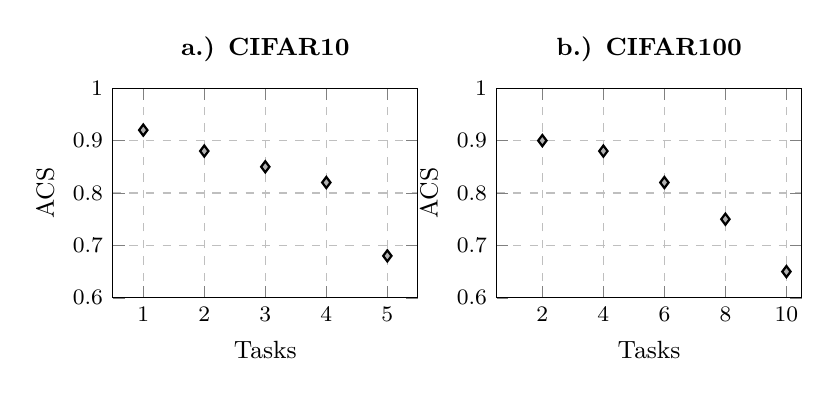
\begin{tikzpicture}
        % Subplot a.) CIFAR10
        \begin{axis}[
            name=ax1,
            width=0.45\textwidth,
            height=0.35\textwidth,
            xlabel={Tasks},
            ylabel={ACS},
            xmin=0.5, xmax=5.5,
            ymin=0.6, ymax=1.0,
            xtick={1,2,3,4,5},
            ytick={0.6,0.7,0.8,0.9,1.0},
            grid=both,
            grid style={dashed, gray!50},
            every axis plot/.append style={mark options={fill=gray!60}},
            title={\textbf{a.) CIFAR10}},
            legend pos=north east,
            mark size=2pt,
            tick label style={font=\footnotesize},
            label style={font=\small},
            title style={font=\small}
            ]
            
            % Data points for CIFAR10
            \addplot[
                only marks,
                mark=diamond*,
                color=black,
                mark options={solid, fill=gray!60},
                dotted,
                thick
            ] coordinates {
                (1, 0.92)
                (2, 0.88)
                (3, 0.85)
                (4, 0.82)
                (5, 0.68)
            };
        \end{axis}
        
        % Subplot b.) CIFAR100
        \begin{axis}[
            name=ax2,
            at={(ax1.south east)}, 
            anchor=south west,
            xshift=1cm,
            width=0.45\textwidth,
            height=0.35\textwidth,
            xlabel={Tasks},
            ylabel={ACS},
            xmin=0.5, xmax=10.5,
            ymin=0.6, ymax=1.0,
            xtick={2,4,6,8,10},
            ytick={0.6,0.7,0.8,0.9,1.0},
            grid=both,
            grid style={dashed, gray!50},
            every axis plot/.append style={mark options={fill=gray!60}},
            title={\textbf{b.) CIFAR100}},
            legend pos=north east,
            mark size=2pt,
            tick label style={font=\footnotesize},
            label style={font=\small},
            title style={font=\small}
            ]
            
            % Data points for CIFAR100
            \addplot[
                only marks,
                mark=diamond*,
                color=black,
                mark options={solid, fill=gray!60},
                dotted,
                thick
            ] coordinates {
                (2, 0.90)
                (4, 0.88)
                (6, 0.82)
                (8, 0.75)
                (10, 0.65)
            };
        \end{axis}
    \end{tikzpicture}
    \caption{Illustration of the Average Confidence Score (ACS) for unlabeled data across tasks. The ACS is calculated by taking the average of maximum probability confidence scores from all the unlabeled data at the end of training. The observed decaying trend indicates that using a fixed high threshold in SS-CIL may not be suitable for effective utilization of unlabeled data in feature learning. Due to the fixed threshold, the amount of unlabeled data utilized for training is significantly reduced as tasks progress.}
    \label{fig:acs_trend}
\end{figure}

\end{document}